\documentclass[landscape,xcolor={table}]{beamer}

\usepackage{amsmath}
\usepackage{graphicx}
\usepackage[english]{babel}
\usetheme{Antibes}
\usepackage{tikz}
\usepackage{multimedia}
\usepackage{textpos}
\usepackage{hyperref}
\usepackage{url}

\usetheme{default}
\usecolortheme{seahorse}
\usefonttheme[onlymath]{serif}
\setbeamertemplate{caption}[numbered]
\graphicspath{ {images/} }

\pgfdeclareimage[width=\paperwidth]{mybackground}{images/blue_sun.png}
\pgfdeclareimage[width=0.2\paperwidth]{rocket}{images/launch}

\setbeamertemplate{title page}{

        \begin{picture}(0,0)

            \put(-30,-250){%
                \pgfuseimage{mybackground}
            }

            \put(-168,-100){%
                \begin{minipage}[b][45mm][t]{226mm}
                
                	\centering
               
                  {\usebeamerfont{title}\color{red}\inserttitle \par}
                  
                  \color{red}\insertauthor
                  
                  \insertinstitute
                  
                  \insertdate
                  
                
                  
                \end{minipage}
            }

            \end{picture}
            
            \begin{textblock*}{100mm}(-0.75cm,-3.5cm)
            
\includegraphics[width=2cm]{images/nasa}
            \end{textblock*}

            \begin{textblock*}{100mm}(0.90\textwidth,-3.75cm)
            
\includegraphics[width=2cm]{images/inverted_solar_physics_logo}
            \end{textblock*}

    }

\title[...]{
\includegraphics[width=2cm]{images/moses_logo_with_text}  \\Hardware and Software Development for \\ MOSES II Flight Operations}
\author[Smart, Remington]{Roy Smart \and Jackson Remington}
\institute{
\includegraphics[width=2cm]{images/msu}}
\date{May 1st, 2015 \\ }

\addtobeamertemplate{frametitle}{}{%
\begin{textblock*}{100mm}(.45\textwidth,-1.7cm)

\includegraphics[width=2cm]{images/nasa} \;

\includegraphics[width=2cm]{images/msu}	\;

\includegraphics[width=2cm]{images/ssel}
\end{textblock*}}

	
\begin{document}

	\begin{frame}[plain]
	        \titlepage
	\end{frame}
	
	\begin{frame}
		
		\frametitle{MOSES Scientific Goals}
		
		\begin{columns}[T] % align columns
		\begin{column}{.48\textwidth}

			\begin{itemize}
				\item hey!
			\end{itemize}
			
		\end{column}%
		\hfill%
		\begin{column}{.48\textwidth}
		
			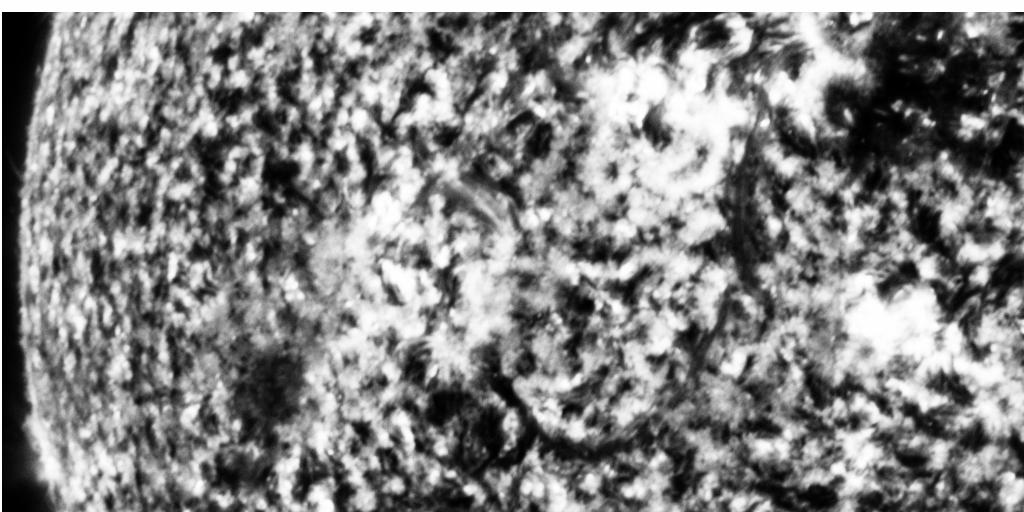
\includegraphics[width=\textwidth]{images/exp2} \\
			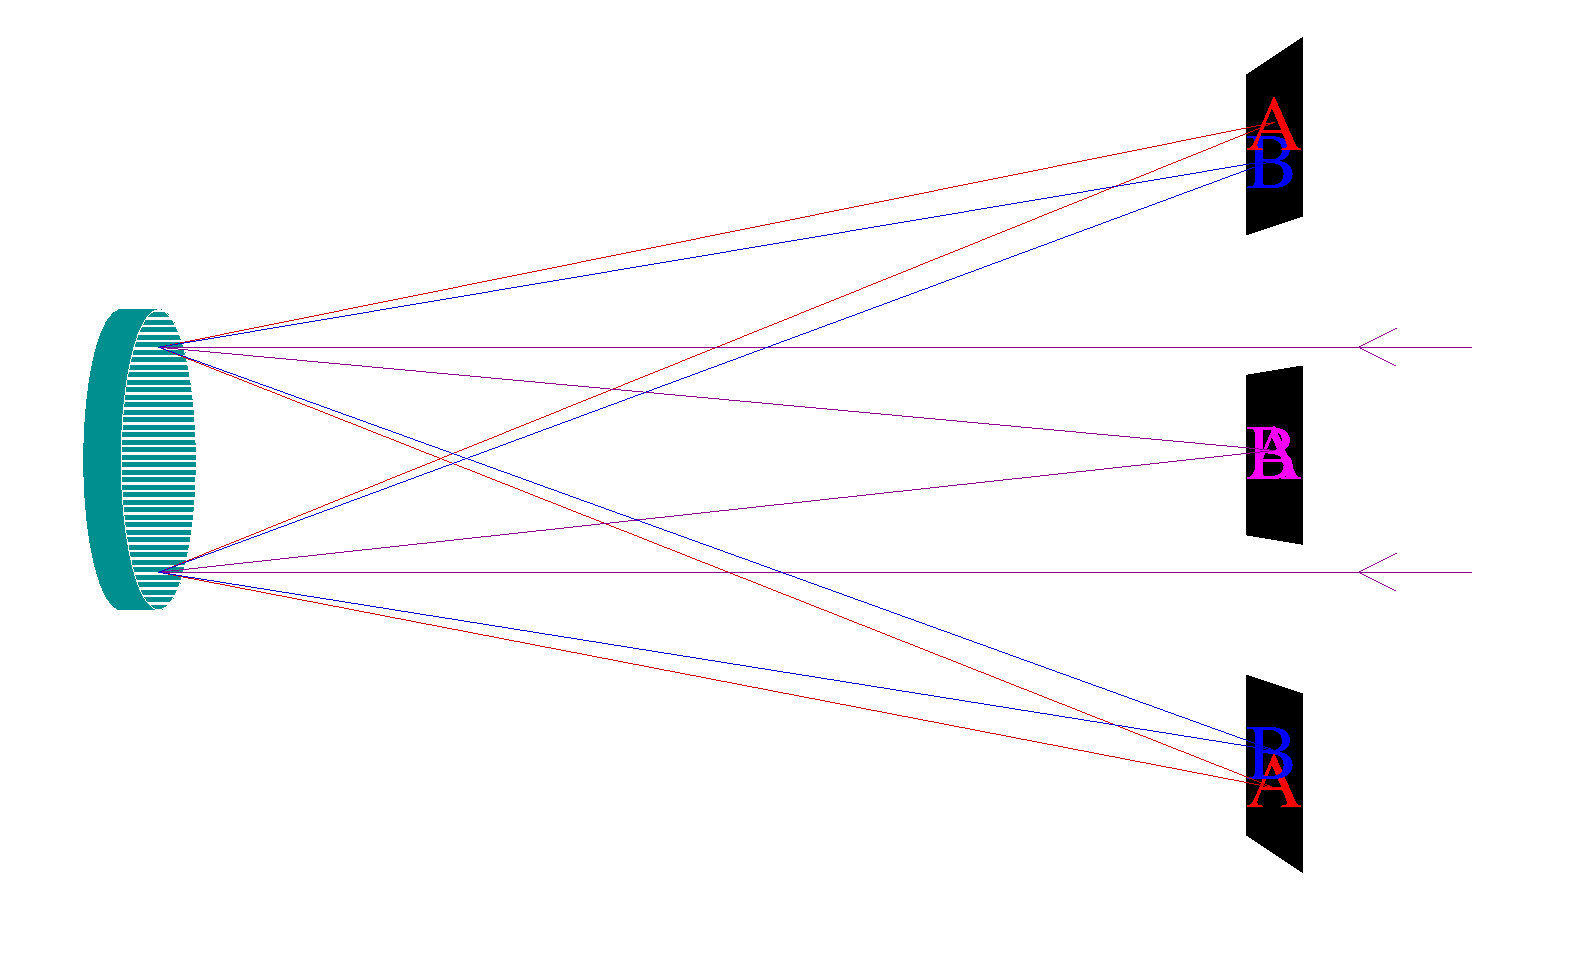
\includegraphics[width=\textwidth]{images/instrument}
		
		\end{column}%
		\end{columns}

	\end{frame}
	
	\begin{frame}
		
		\frametitle{First Launch}
		
		\begin{columns}[T] % align columns
		\begin{column}{.20\textwidth}

			\movie[width=3cm,height=7cm,poster,externalviewer]{\pgfuseimage{rocket}}{images/Launch.mp4}
			
		\end{column}%
		\hfill%
		\begin{column}{.78\textwidth}
		
			\begin{itemize}
				\item MOSES first launched in February 8th, 2006 \cite{moses}.
				\begin{itemize}
					\item Utilized a Black Brant IX sounding rocket
					\item Observed the Sun in He II 304 \AA
					\item Identified a Transition Region Explosive Event.
					\item Payload was retrieved with data intact.
					\item Flight computer was damaged after launch. We hypothesize that it was damaged after splashdown into atmosphere.
				\end{itemize}
				
			\end{itemize}
		
		\end{column}%
		\end{columns}
	
	\end{frame}
		
	\begin{frame}
	
		\frametitle{System Requirements}
		
				\begin{columns}[T] % align columns
				\begin{column}{.49\textwidth}
					\begin{itemize}
						\item Data characteristics
						\begin{itemize}
							\item MOSES captures the sun in three spectral orders $m=-1,0,1$.
							\item Each spectral order is captured by CCDs at $2048 \times 1024$ resolution.	
						\end{itemize}
					\end{itemize}
					
				\end{column}%
				\hfill%
				\begin{column}{.49\textwidth}
				
					\begin{itemize}
						\item
					\end{itemize}
				
				\end{column}%
				\end{columns}
		
		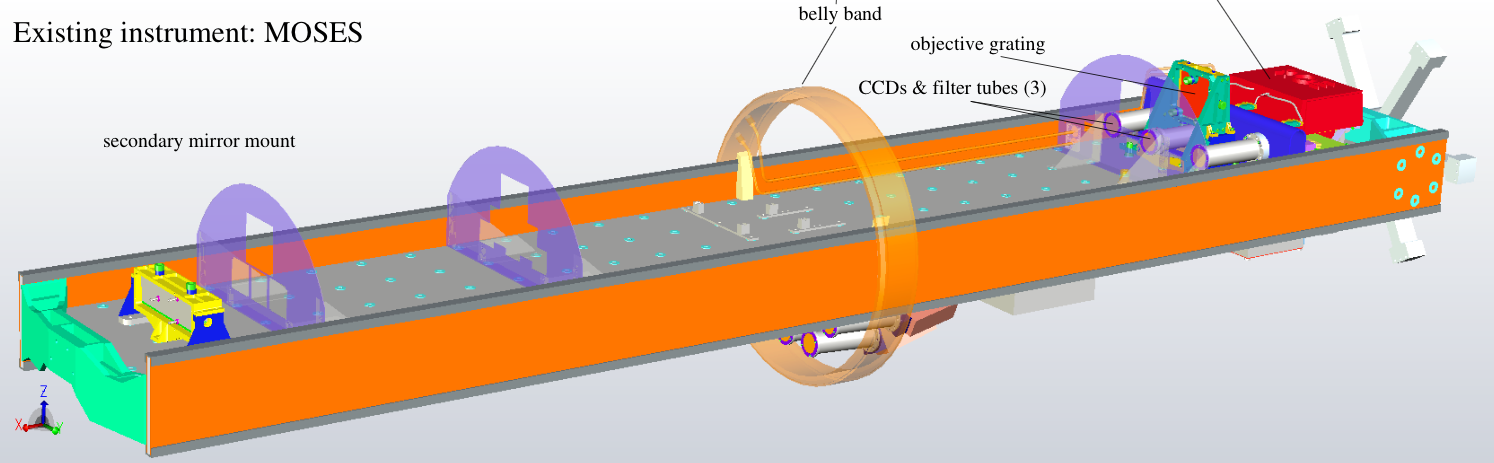
\includegraphics[width=\textwidth]{images/moses}

	\end{frame}
	
	\begin{frame}
		
		\frametitle{Hardware Overview}
		
		\begin{columns}[T] % align columns
		\begin{column}{.68\textwidth}


			
		\end{column}%
		\hfill%
		\begin{column}{.30\textwidth}

			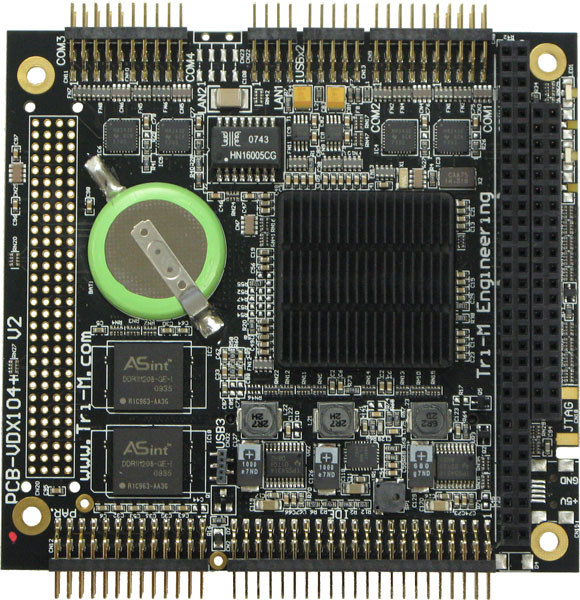
\includegraphics[width=\textwidth]{images/vdx104} \\
			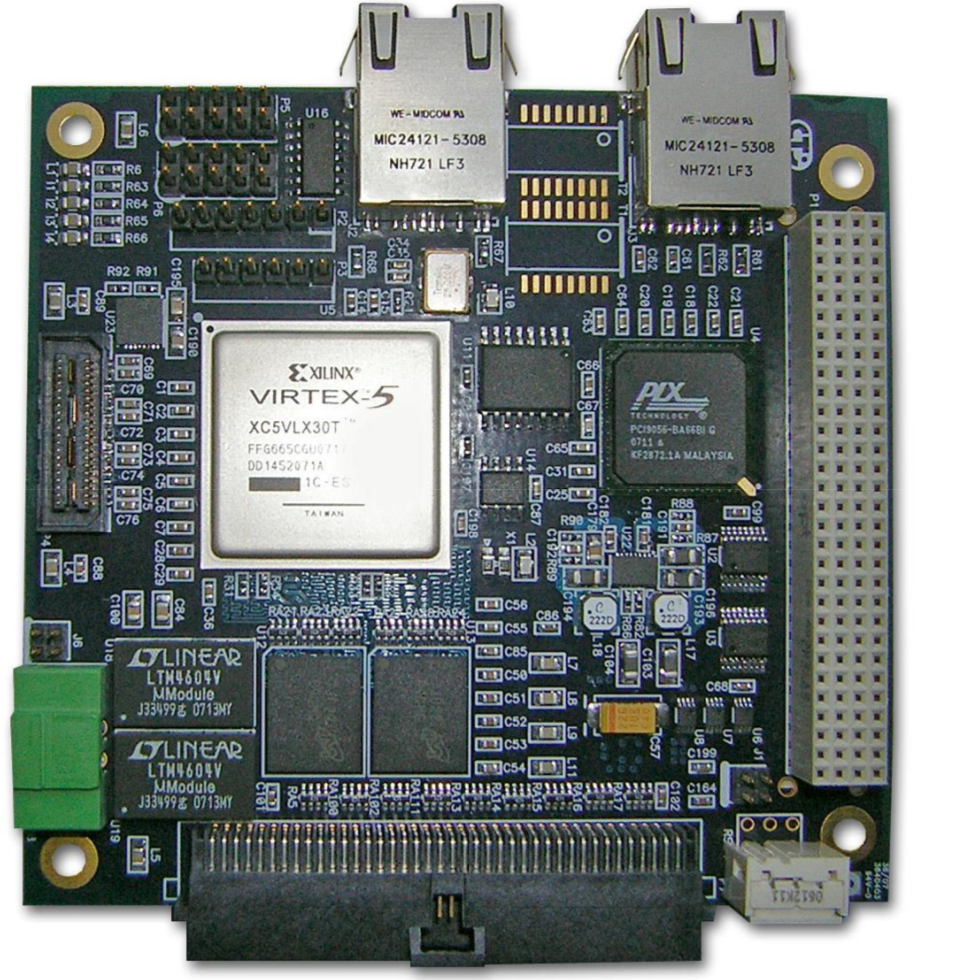
\includegraphics[width=\textwidth]{images/fpga}
					
		\end{column}%
		\end{columns}
			

	\end{frame}
	
	\begin{frame}
		
		\frametitle{Flight Software}
		
		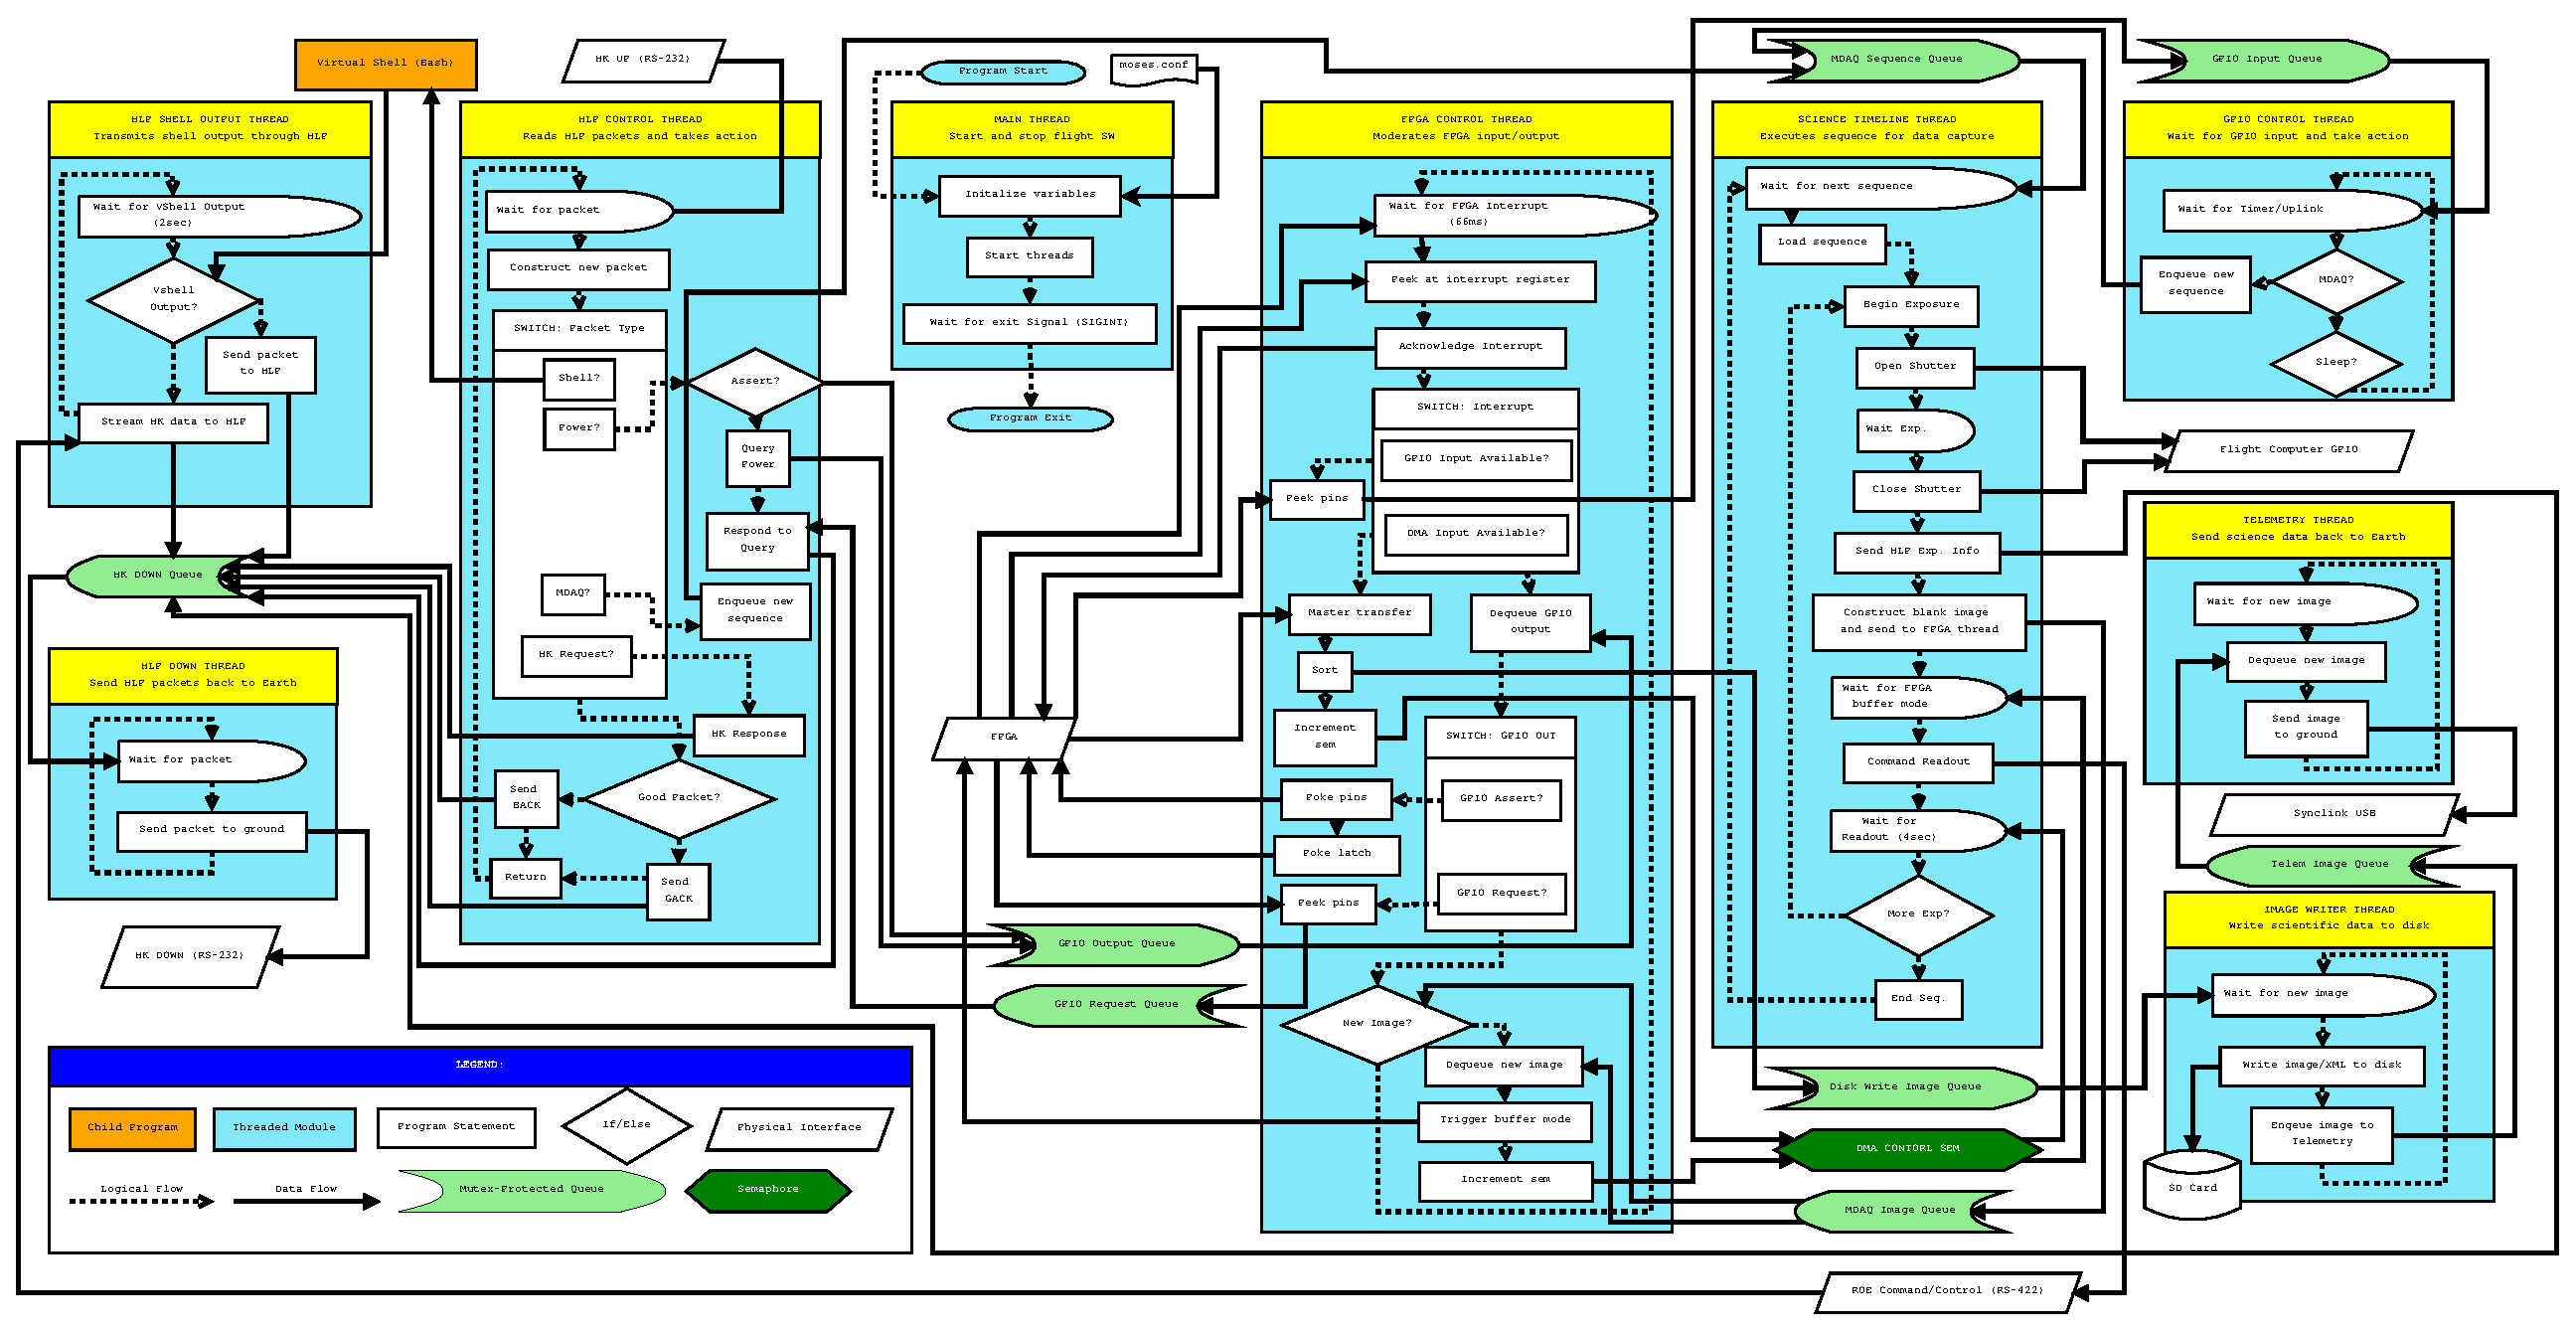
\includegraphics[width=\textwidth]{images/mfsw_block}

	\end{frame}
	
	\begin{frame}
		
		\frametitle{Ground Station Software}
		
		\begin{columns}[T] % align columns
		\begin{column}{.53\textwidth}

			 \begin{itemize}
						  	\item{Server module}
						  	\item{Client module}
						  	\item{Grounded communication}
						  	\begin{itemize}
						  		\item{Serial console}
						  		\item{Ethernet}
						  	\end{itemize}
						  	\item{In-flight communication}
							\begin{itemize}
						  		\item{Housekeeping Link Protocol (HLP)}
						  		\item{Timers}
						  		\item{High-speed telemetry}
						  	\end{itemize}
			 \end{itemize}
			
		\end{column}%
		\hfill%
		\begin{column}{.45\textwidth}

			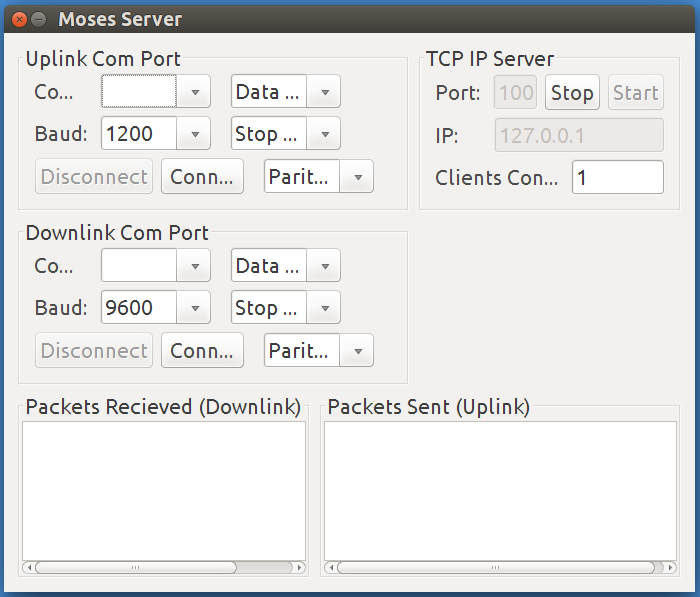
\includegraphics[width=0.7\textwidth]{server_scr} \\
			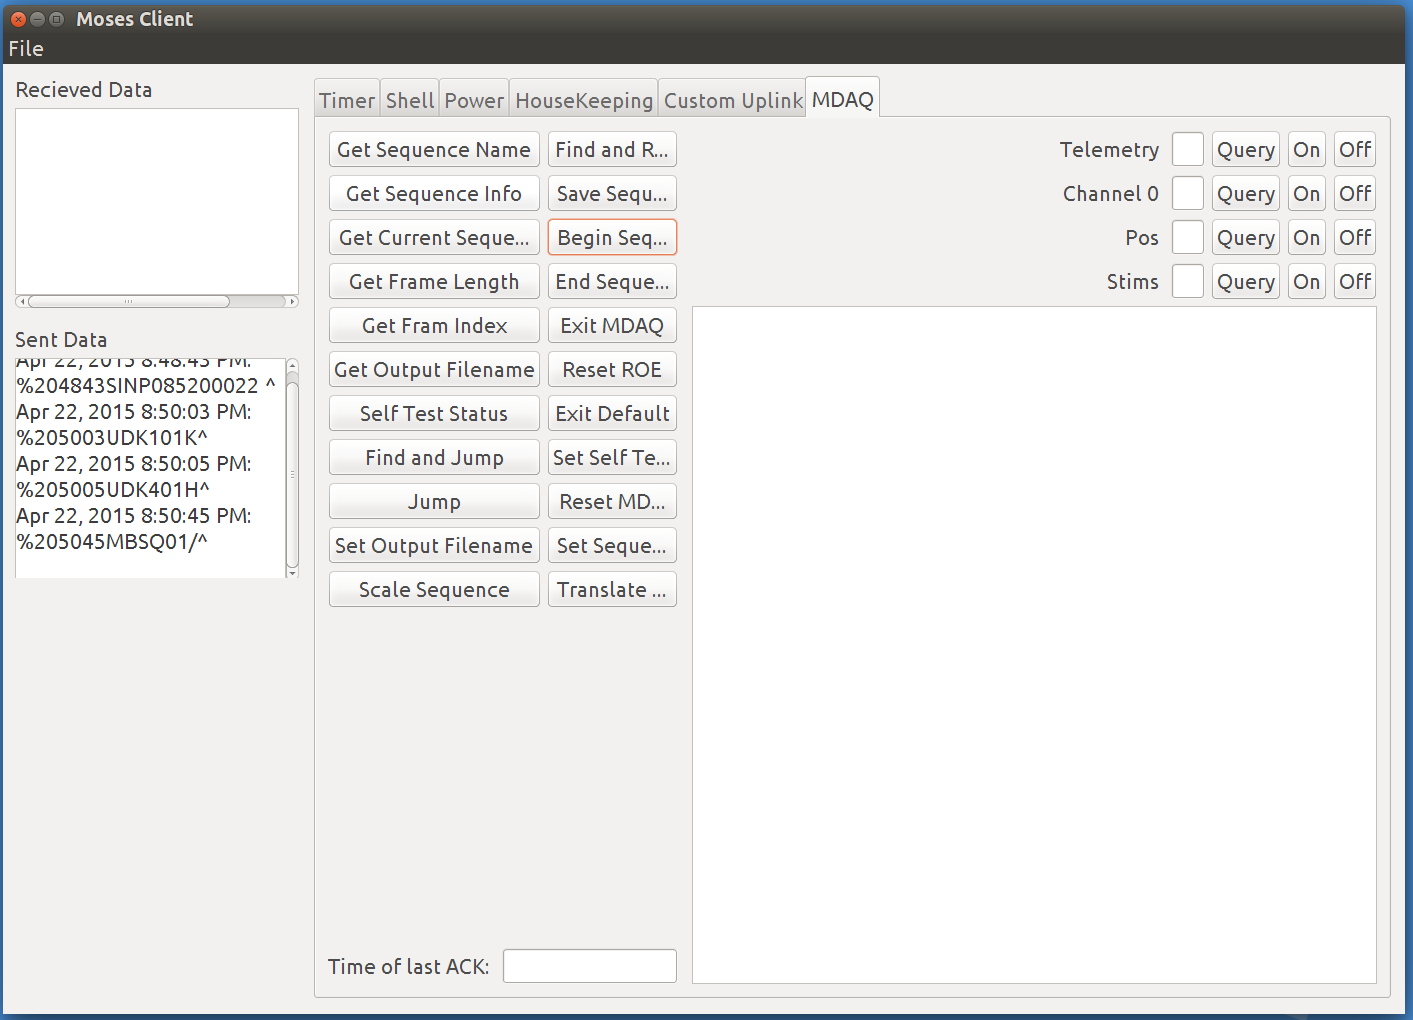
\includegraphics[width=\textwidth]{client_scr}
					
		\end{column}%
		\end{columns}

	\end{frame}
	
	\begin{frame}
		
		\frametitle{Capturing Data}
		
		\begin{columns}[T] % align columns
		\begin{column}{.49\textwidth}

			
\includegraphics[width=\textwidth]{images/selftest_plus} \\
			
\includegraphics[width=\textwidth]{images/stims_zero}
			
		\end{column}%
		\hfill%
		\begin{column}{.49\textwidth}
		
		\end{column}%
		\end{columns}
		

	\end{frame}
	
	\begin{frame}
		
		\frametitle{Data Retrieval}
		
		\begin{columns}[T] % align columns
		\begin{column}{.49\textwidth}

			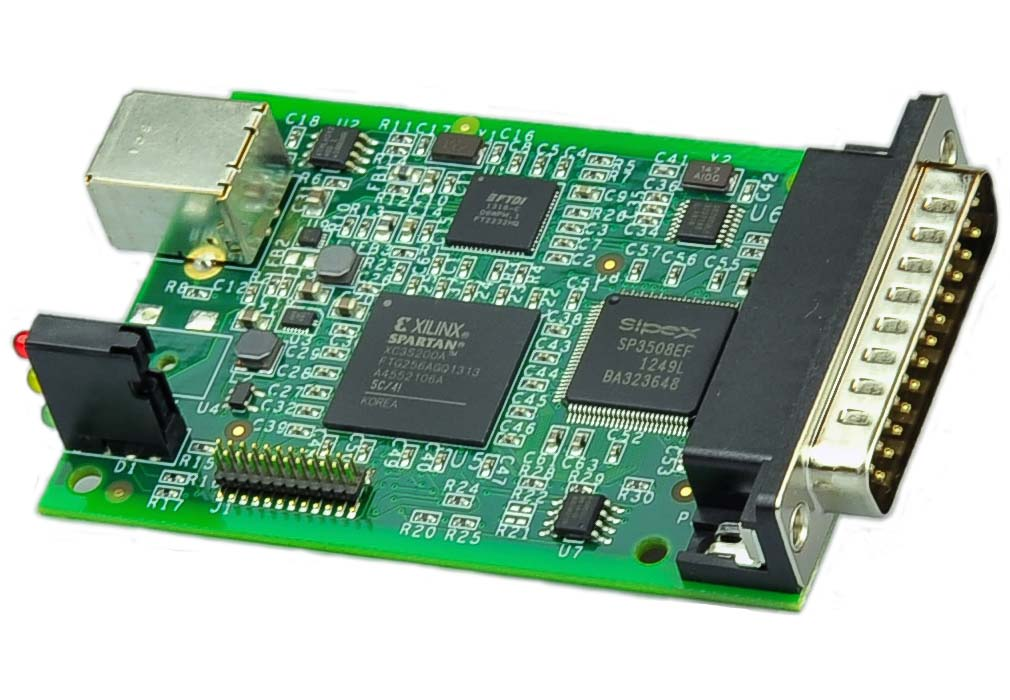
\includegraphics[width=0.5\textwidth]{images/synclink} \\
			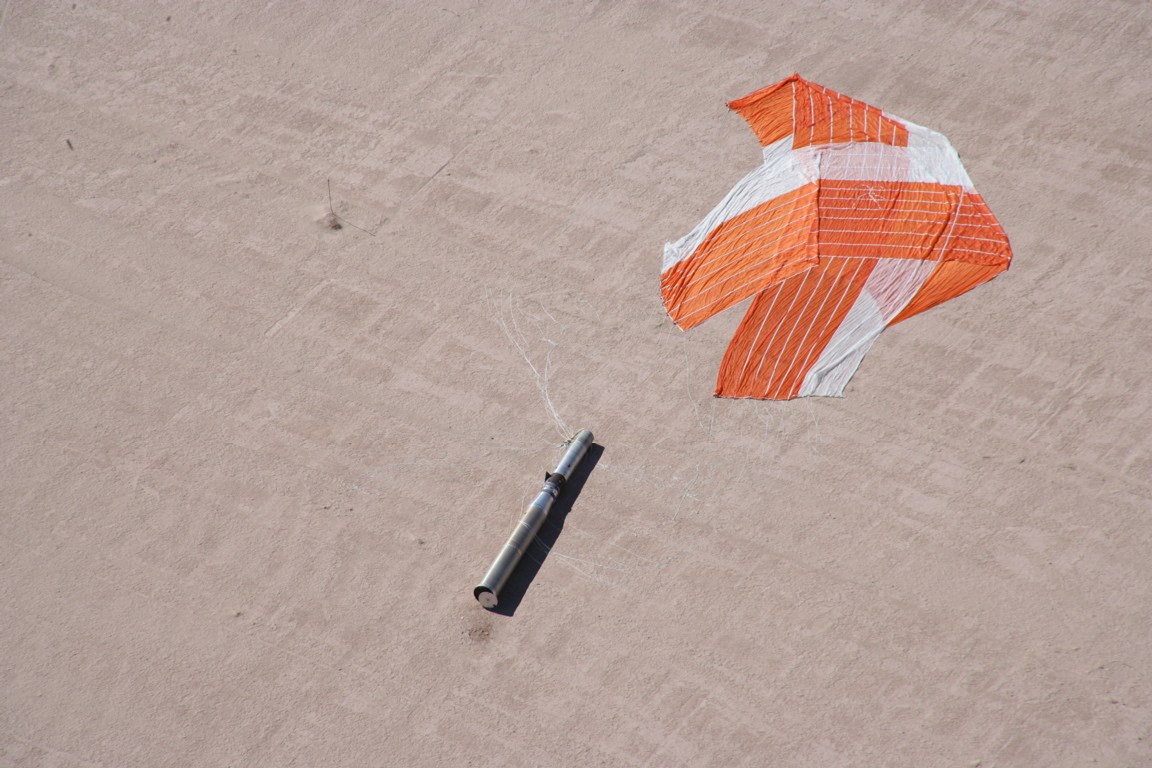
\includegraphics[width=\textwidth]{images/desert}
			
		\end{column}%
		\hfill%
		\begin{column}{.49\textwidth}


					
		\end{column}%
		\end{columns}

	\end{frame}
	
	\begin{frame}
		
		\frametitle{Next Launch}
		
		\begin{columns}[T] % align columns
		\begin{column}{.49\textwidth}

			
			
		\end{column}%
		\hfill%
		\begin{column}{.49\textwidth}

			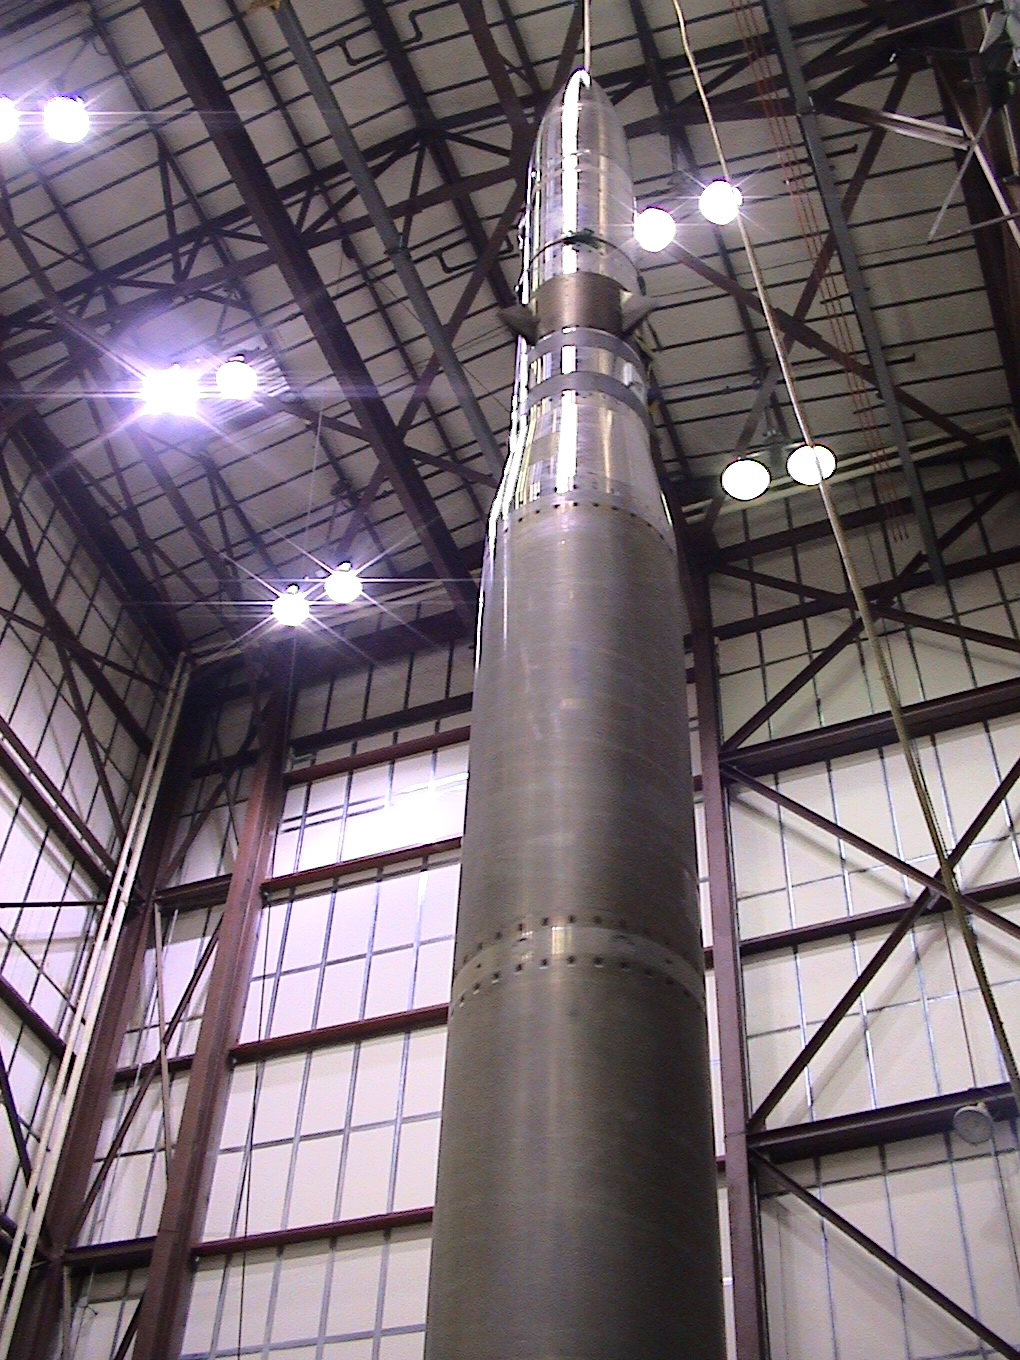
\includegraphics[width=\textwidth]{images/high}
					
		\end{column}%
		\end{columns}

	\end{frame}
	
	\begin{frame}
		\frametitle{References}
		
		\bibliographystyle{unsrt}
		\bibliography{sources}
	\end{frame}
	
\end{document}








